\section{Introduction}
% Short abstract introduction here about this section (can be done when finished)

\subsection{Background}
\label{introduction-background}
% What is SeaDataCloud's exact problem? Make the problem clear so that our solution fits the problem. Try to look at it from all angles, like an os3 teacher would

% European Open Science Cloud
Research clouds such as proposed in the \gls{eosc} will offer Europe's 1.7 million researchers and 70 million science and technology professionals the means to store, share and re-use large volumes of information generated by the big data revolution \cite{eurocloud}. Research clouds publish datasets from distributed sources, identified by a \gls{pid} (more details in section \ref{pid-intr}). These datasets are not accessed via e.g. a simple web portal like traditional internet objects on the web. Instead these requests are processed by e.g. a data catalog of the federated research cloud. Therefore, research clouds face the challenge of identifying distributed data in a federated cloud, provide data provenance and provide a scalable service to serve many users that request large datasets.

Furthermore, research clouds face a trend of increased data production and consumption, which is expected to grow. This general trend in research clouds calls for a data distribution solution that better supports the scale and complexity. In this section we will briefly discuss the technical challenges.

An example of such a research cloud is SeaDataNet, which is a distributed marine data infrastructure network for managing the large and diverse data sets collected by the oceanographic fleets and the automatic observation systems. SeaDataNet started the SeaDataCloud project in 2016. Their aim is to advance and increase the usage of SeaDataNet's services by adopting cloud and high performance computing technology for better performance \cite{sdc}. Their current infrastructure is a centralized solution (figure \ref{fig:sdc_cur}), as the current cache is a central catalogue which duplicates the entire data repository.

\begin{figure}[H]
\centering
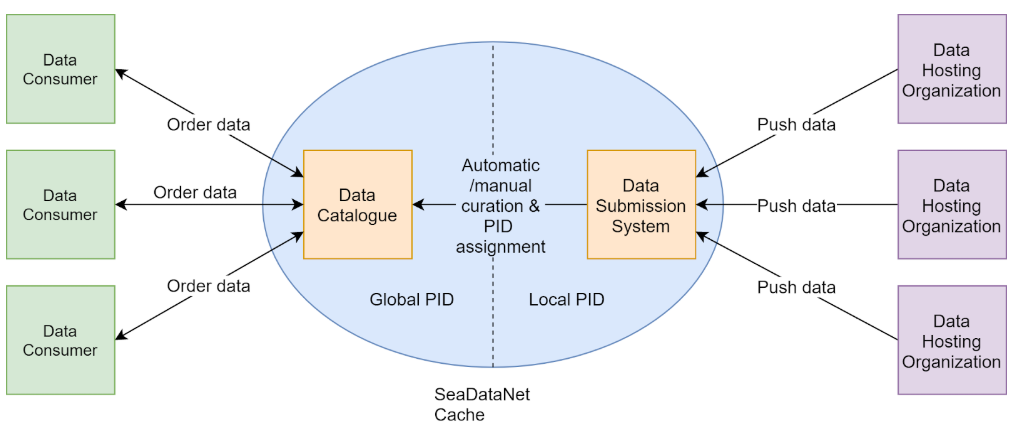
\includegraphics[scale=0.57]{Images/SDC_current.png}
\caption{SeaDataCloud's current infrastructure.}
\label{fig:sdc_cur}
\end{figure}

Data consumers use host-to-host-connections (IP) to pull data from this cache, which could cause congestion with many concurrent data consumers. SeaDataCloud aims at considerably advancing SeaDataNet services and increasing their usage, more users are expected to be engaged and for longer sessions \cite{sdc-eu}.
 
Another research cloud example is \gls{cs3}, which is a data infrastructure that brings together users, researchers, developers, technology, and service providers of on-premise cloud services as well as large cloud service companies \cite{cs3}. The \gls{cs3} community has been growing for the last three years and currently includes around one hundred institutions and companies from around the world.

The general problem that can be subtracted from figure \ref{fig:sdc_cur} is that research clouds face a potential congestion problem, and thus network and data processing performance degradation when many concurrent data consumers are active. In the field of big science (big data), several data distribution technologies are being experimented with, one of these technologies is \gls{ndn} (more details in section \ref{introduction-ndn}). \gls{ndn} could be a solution to distribute network load and data distribution more efficiently.

% feedback below partially applied, check again
% You should highlight: i) research data infrastructure publishes data from distributed sources, but serve large user communities, ii) such data infrastructure is not a simple web portal of accessing digital objects, but federation of data catalog, repositories and other processing services, iii) research data face challenges of identification, provenance, workflows etc,; the data in the infrastructure is continuously updated, sometimes also from the user. 

% One of the technical challenges is the distribution of the data across the communities. The issue is that the data is distributed by different data providers across these communities, each with their own naming schema. Therefore, interoperability across different naming schemas has to be achieved. Users should be able to request data across these communities, without having to cope with different schemas for data they request. Another technical challenge is to serve this data to a large number of users. 

% The current approach can potentially cause congestion and delays with many concurrent users consuming data from the highlighted distributed data infrastructures. On top of that, the large number of users is still growing. In section \ref{tech-oview} we highlight state of the art technologies to deal with these challenges. We will create a design which achieves interoperability across different naming schemas and alleviates network latency and congestion.

% stuff below is not true i suppose, this interoperability only becomes an issue when ndn is introduced. pid schemas work just fine together.
% One of the most important topics and technical challenge of \gls{cs3} services is interoperability of the different naming schemes being used to identify data. Development of interoperability protocols is important to provide data sharing capabilities for all users across all institutions in the field of education and research.

\subsection{Research question}
\label{introduction-research-question}
% Based on the use case and related work, what is it that we will research and why? What is it that we want to answer?
With the technical challenges and problem statement in mind, as described in section \ref{introduction-background}, we will answer the following questions which are divided into two main research questions.

\begin{enumerate}
	\item A translation is needed between the \gls{pid} and \gls{ndn} namespace in order to make these solutions compatible, thus; how to make the \gls{pid} and \gls{ndn} namespace interoperable?
\end{enumerate}

We will research different \gls{pid} types to find a feasible approach to implement \gls{ndn} interoperability with extensibility in mind for \gls{pid} types.

%This is in response to the highlighted data infrastructures described in section \ref{introduction-background}, which cope with interoperability across different data providers. This is due to the fact that the different data providers use different naming schema to serve objects to data consumers.

%Next to this, SeaDataCloud's planned solution needs to support multiple \gls{pid} types, as \glspl{pid} that get assigned to objects in their infrastructure can be of any type, we will look into supporting different \gls{pid} types to find a feasible solution to implement future \gls{pid} types easily. This will be answered with the following sub-questions.
\begin{itemize}
    \item[--] How to support different \gls{pid} types?
    \item[--] How to incorporate extensibility for future \gls{pid} schemas?
\end{itemize}

The problem statement discussed in \ref{introduction-background} calls for a data distribution solution. Therefore, we will research the planning and deployment of an \gls{ndn} with scalability in mind. To achieve this, the following research question needs to be answered.
\begin{enumerate}
\setcounter{enumi}{1}
    \item How to plan and manage an \gls{ndn}'s life cycle with scalability in mind?
\end{enumerate}

To answer this research question we need to analyze the known scalability problems in \gls{ndn}. Furthermore, the term scalability needs to apply to manageability as well. If scaling in or out in terms of resources is made uncomplicated, the efforts needed to manage this infrastructure needs to stay the same.
\begin{itemize}
    \item[--] Which \gls{ndn} scaling problems are known?
    \item[--] Which method can be used to plan an NDN?
    \item[--] How to deploy an \gls{ndn} with scalability in mind?
\end{itemize}

\subsection{Scope}
\label{introduction-scope}
% What will we do and what will we skip? Based on what's already done in related work and our research question

% related work (section \ref{introduction-related-work}) and

Based on the research question we defined the following scope. We will develop a method to make the \gls{pid} types \gls{urn}, Handle and \gls{doi} interoperable with the \gls{ndn} namespace. This will be done to demonstrate that interoperability of different \gls{pid} types is possible within \gls{ndn}. The reason we do not cover more \gls{pid} types in our methodology is because with the aforementioned \gls{pid} types we can already prove that \gls{pid} interoperability is possible. Therefore, the interoperability goals are to demonstrate that different \gls{pid} types can be used within \gls{ndn}.

The planning of the \gls{ndn} has the following goals. We did not have access to performance monitoring data from research clouds such as SeaDataCloud or \gls{cs3}. Thus, a starting baseline will be determined based on the known performance limitations (section \ref{introduction-related-work-ndn}) and the problem statement discussed in section \ref{introduction-background}. Using this starting baseline, a method will be developed for \gls{ndn} planning and deployment. This includes a proof of concept where, based on \gls{ndn}'s adaptability, the network can be adjusted for scale in both performance but also in terms of manageability. The proof of concept will be limited to existing software solutions. Therefore, solutions that are still in a research or development phase and not yet implemented or made public will not be explored in the proof of concept. The proof of concept will be setup in a small scale and is used to demonstrate the methods and train of thought used to deploy the \gls{ndn} with the mentioned scalability properties. However, the methods developed should be applicable to also larger deployments (research clouds) without alternation.

\subsection{Report structure}
This report is structured as follows; after the background of this research is discussed, the research questions are presented. This research is divided into two research parts, each with their own scope and results. Related work will be discussed in section \ref{introduction-related-work}. A technical background is provided in section \ref{tech-oview}. These technical details assist in understanding our methods and technology choices we made to answer the research questions. These technologies are used in our methodology sections; \ref{pid-poc} and \ref{planning-ndn}. These methods are tested in a proof of concept. The results of both methods in the proof of concept will be summarized and the novelty evaluated in the discussion (section \ref{disc}). Furthermore, we also discuss preliminary performance results based on our proof of concept in section \ref{discussion-performance}. We will conclude our findings and provide future work in section \ref{fut}. Uncommon acronyms are listed in the appendix in section \ref{appendix}.



% After introducing the concepts and related work of our research subjects, we will continue to discuss the technical background in section \ref{tech-oview}. In this technical background we will explore \glspl{pid}, \gls{ndn}, McCabe, \gls{tosca} and virtualization in more detail with the research scope in mind.  Our methodology in sections \ref{pid-poc} and \ref{planning-ndn} provide a prototype for demonstrating the planning and scaling of an \gls{ndn} with \gls{pid} interoperability. For \gls{pid} interoperability with the \gls{ndn} namespace we will also focus on the ease of extensibility for future \gls{pid} types. Our interoperability approach is integrated in our proof of concept which makes use of the planning and scaling methods of section \ref{planning-ndn}. By combining these methods we will be able to demonstrate that the consumer can still retrieve objects from the producer, despite scaling the \gls{ndn} in our out. And thus provides data distribution by the use of \gls{ndn}, which in turn lowers the chance of network congestion for e.g. research clouds. Furthermore, we will discuss our combined methods in more detail in section \ref{disc}, where 
